\section{Algorithm}

In this section we describe the components of our algorithm and their
relationship with each other.  The algorithm predicts the syntactic
category of a word in a given context based on its substitutes.  In
other words first we construct the co-occurrence representation of
words and their substitutes with the help of a language model and then
map each value in the co-occurrence data to a corresponding embedding
on a $n$ dimensional sphere using the S-CODE algorithm.  Finally, we
apply k-means clustering to categorize the word embeddings by which we
induced the word categories.  In the next subsection we detail the
construction of co-occurrence representation of the input, in
Subsection~\ref{sec:cooc} we explain the embedding calculation and
finally in Subsection~\ref{??} we describe the different ways of
embedding clustering.

\subsection{Co-occurences}
\label{sec:cooc}
% How we represent the context?
% How we relate the word and the context?

Word contexts are represented by substitutes sampled from the
corresponding substitute word distributions.  Substitute words are
sampled with replacement from the substitute distributions that are
calculated based on an n-gram language model.  The sample space of the
substitute word distributions is the vocabulary of the language
model.\footnote{Sampled substitutes might include the unknown word tag
  ``\_unk\_'' since it is in the language model vocabulary.  For
  example substitutes of proper nouns usually include ``\_unk\_'' as a
  substitute.}  It is possible (and beneficial, see
Section~\ref{sec:exp}) to sample more than one substitutes (see
Table~\ref{tab:samples}) and generate more pairs from the same
substitute distribution.  The calculation of substitute distributions
and substitute sampling are detailed in Appendix~\ref{sec:subcomp}.
To capture the relation between each word and its context we construct
a co-occurrence representation by pairing the words with their sampled
substitutes.  Table~\ref{tab:samples} shows sampled substitutes of
each word and their co-occurrence representation on an example
sentence.  A word might appear as a target word or a sampled
substitute therefore to clarify this ambiguity we concatenate ``W''
and ``S'' to words and substitutes, respectively, on the co-occurrence
data.

The next section explains the S-CODE algorithm which takes the
co-occurrence data as its input and calculates the embeddings of the
words and their substitutes on an $n$ dimensional sphere.  In the rest
of paper we use the term ``substitutes'' to refer ``sampled
substitutes''.

\begin{table}[ht]
\caption{The left table shows three possible substitutes, seperated
  with ``/'', sampled for each of the positions in the example
  sentence \textit{``Pierre Vinken, 61 years old, will join the board
    as a nonexecutive director Nov.~29 .''} based on a 4-gram language
  model.  The right table represents the input sentence as a
  co-occurrences of words and their substitutes.  Thus words on the
  left column represents the target word while words on the right
  column represents the context of the correponding target word.}
\begin{tabular}{|ll|} \hline
\textbf{Word} & \textbf{Sampled Substitutes}\\
\hline
Pierre & \textit{Mr.}  / \textit{Pierre} /  \textit{Mr.}\\
Vinken & \textit{\_unk\_} / \textit{Beregovoy} / \textit{Cardin}\\
, & \textit{,} / \textit{,} / \textit{,}\\
61 & \textit{48} / \textit{52} / \textit{41}\\
years & \textit{years} /  \textit{years} /  \textit{years}\\
old & \textit{old} /  \textit{old} /  \textit{old}\\
, & \textit{,} /  \textit{,} /  \textit{,}\\
will & \textit{will} /  \textit{will} /  \textit{will}\\
join & \textit{head} /  \textit{join} /  \textit{leave}\\
the  & \textit{its} /  \textit{its} /  \textit{the}\\
board & \textit{board} /  \textit{company} / \textit{firm}\\
as & \textit{as} / \textit{as} / \textit{as}\\
a & \textit{a} / \textit{a} / \textit{a}\\
nonexecutive & \textit{nonexecutive} / \textit{non-executive} / \textit{nonexecutive}\\
director & \textit{chairman} / \textit{chairman} / \textit{director}\\
Nov. & \textit{April} / \textit{May} / \textit{of}\\
29 & \textit{16} /  \textit{29} / \textit{9}\\
. & \textit{.}  / \textit{.} / \textit{.}\\
\hline
\end{tabular}
\quad
\begin{tabular}{|ll|}
\hline
\textbf{Word} & \textbf{Substitute}\\
\hline
W:Pierre & \textit{S:Mr.}\\
W:Pierre & \textit{S:Pierre}\\
W:Pierre & \textit{S:Mr.}\\
W:Vinken & \textit{S:unk}\\
W:Vinken & \textit{S:Beregovoy}\\
W:Vinken & \textit{S:Cardin}\\
$\hdots$&\\
W:join & \textit{S:head}\\
W:join & \textit{S:join}\\
W:join & \textit{S:leave}\\
W:the & \textit{S:its}\\
W:the & \textit{S:its}\\
W:the & \textit{S:the}\\
$\hdots$&\\
W:director & \textit{S:chairman}\\
W:director & \textit{S:chairman}\\
W:director & \textit{S:director}\\
$\hdots$&\\
\hline
\end{tabular}
\label{tab:samples}
\end{table}

\subsection{Co-occurence Embedding}

The S-CODE algorithm maps each word and substitute value in the
co-occurrence data to an embedding on an $n$ dimensional sphere as
detailed in Appendix~\ref{sec:codethr}.  The basic idea of the mapping
is that words and substitutes that are frequently observed as pairs in
the co-occurrence data will have close embeddings while unobserved
pairs will have embeddings that are apart from each other.
\begin{figure}[ht]
\centering
  \begin{minipage}[c]{0.38\textwidth}
    \begin{tabular}{|l|l|}
    \hline
    \textbf{Word} & \textbf{Substitute} \\
    \hline
    $\hdots$&$\hdots$\\
    W:director & S:chairman \\
    W:chief & S:chairman \\
    $\hdots$&$\hdots$\\
    W:Pierre & S:Mr. \\
    W:Frank & S:Mr. \\
    $\hdots$&$\hdots$\\
    \hline
  \end{tabular}
  \end{minipage}
  \begin{minipage}[c]{0.48\textwidth}
    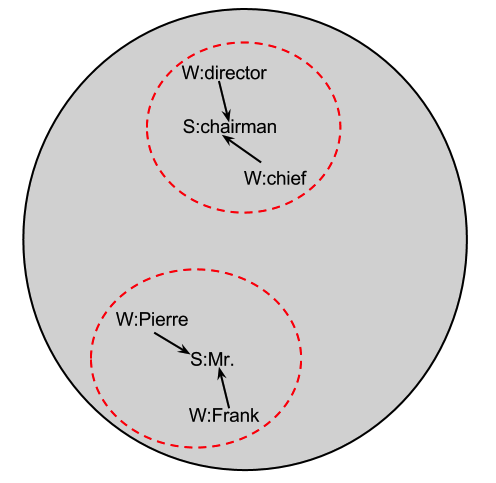
\includegraphics[height=\textwidth]{scode-ex.png}
  \end{minipage}
  \caption{The figure on the right is the final embeddings of the
    input co-occurrence data given on the left table after S-CODE
    converges.  Dashed circles represent the possible groupings of the
    embeddings on the sphere.}
  \label{fig:scodeexample}
\end{figure}

%% \begin{figure}
%% \begin{floatrow}
%% \capbtabbox{%
%% }
%% {%
%%   \caption{A co-occurrence data that
%%  is input to the S-CODE algorithm.}%
%% }
%% \hspace{1cm}
%% \ffigbox{%
%%   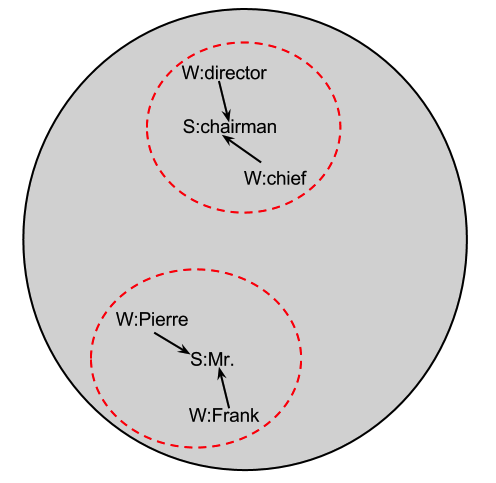
\includegraphics[height=.45\textwidth]{scode-ex.png}\\  
%% }
%% {%
%%   \caption{}  
%%   \label{fig:scodeexample}
%% }
%% \end{floatrow}
%% \end{figure}

The sample co-occurrence data in Figure~\ref{fig:scodeexample}
consists of pairs such as (\textit{W:director}, \textit{S:chairman})
and (\textit{W:chief}, \textit{S:chairman}) therefore S-CODE forces
the embeddings of \textit{W:director} and \textit{W:chief} to be close
to the embedding of \textit{S:chairman}.  Similar to the former case
the embeddings of \textit{W:Pierre} and \textit{W:Frank} will be close
to the embedding \textit{S:Mr.} due to the frequently observed pairs.
As a results the final embeddings of \textit{W:director} and
\textit{W:chief} will be close to each other due to the common
substitute \textit{S:chairman} and will be apart from
\textit{W:Pierre} and \textit{W:Frank} due to the lack of common
substitute as shown on Figure~\ref{fig:scodeexample} (similarly the
embeddings of \textit{W:Pierre} and \textit{W:Frank} will be close to
each other due to \textit{S:Mr.}).

% How we relate final embeddings and the input pairs?
S-CODE constructs embeddings on $n$ dimensional sphere for each unique
value of words and substitutes.  Thus each pair in the co-occurrence
data can be represented in three different ways by using the output of
S-CODE: (1) word embedding (${\bf W}$) which represents the type
information, (2) substitute embedding (${\bf S}$) which represents the
context information, and (3) word and substitute embeddings
concatenated (${\bf W}\oplus{\bf S}$).  In the next section we apply
k-means clustering to these three representation and analyze the
characteristic of final clusters.

\subsection{Co-occurrence Embedding Clustering}

%% In Section~\ref{sec:cooc} we decribe the tranformation of an input
%% sentence to a co-occurrence data and we represent each target word
%% with the word--substitute pair(s).  In the previous section we
%% construct embeddings for each value observed in the co-occurrence data
%% using the S-CODE algorithm. 

Each target word in the original input sentence is represented with
word--substitute pairs and each unique word and substitute value are
represented with embeddings on an $n$ dimensional sphere.  Therefore
clustering the embeddings means clustering the target words in the
original input.  We run instance weighted k-means algorithm to cluster
the final embeddings constructed by S-CODE.  The target words can be
represented in three ways as described in the previous section.

\paragraph{Word embeddings (${\bf W}$)}  In this representation all
instances of the target word in the data is represented with the same
embedding thus clustering based on these embeddings employ the
one-tag-per-word assumption from the beginning.  For example, in
Table~\ref{tab:samples} eventhough we sample three substitutes per
target word, each unique target word has only one embedding in ${\bf
  W}$.

\paragraph{Substitute embeddings (${\bf S}$)}  In this representation 
each target word instance is represented with its substitutes
embeddings thus clustering them does not employ or force the
one-tag-per-word assumption.  For example, in Table~\ref{tab:samples}
the word \textit{W:Pierre} will be represented with the embeddings of
{\it S:Mr.} {\it S:Pierre} and {\it Mr.}.  K-means might cluster
substitute embeddings into different clusters which creates an
ambiguity on the final cluster of the target word.  To solve this
issue the target word is assigned to the cluster in which the majority
of its substitute embeddings are present\footnote{Ties are broken
  randomly}.

%% For example each unique target word in our example sentence given on
%% Table\ref{tab:samples} has only one correponding embedding in ${\bf
%%   W}$ thus clustering the correponding embeddings of the target words
%% means clustering the target words.  However the situation is a little
%% bit trickier when we represent the target word with ${\bf S}$ or ${\bf
%%   W}\oplus{\bf S}$
